


        
        \section{Neutron stars in binary systems}
        \label{binary_NS}

            Astrophysical prospects for binary pulsar detection. 
            Binary pulsars are perhaps our best hope for detecting continuous gravitational waves.

            \subsection{Binary spin-up and detectable lifetime}
            \label{spin-up}
         
                GW pulsar lifetime alone vs companion.

            \subsection{Detection rate projections}
            \label{rate_projections}

                aLIGO rate projections.

        \section{TwoSpect all-sky searches}
        \label{all-sky}

            TwoSpect methods as-is. These are described in detail in Evan Goetz's thesis~\cite{GoetzThesis}. Note that the code is located on the web freely accessible in the LALApps repository~\cite{LALAPPSrepo}.

            \subsection{Two spectra: a double Fourier transform}
            \label{two_spectra}

                'Two spectra' -- FFT of periodograms reveals modulation of sine waves.

            \subsection{Infering neutron stars with companions}
            \label{inference}
 
                Infer whether modulation is due to a companion star.

        \section{Scorpius X-1 and results from Directed TwoSpect}
        \label{directed_results}
 
            Preliminary results of a directed search (possibly simulation-only).

            We have a great deal of material here already, just need to pull from figures and commentary from the Sco X-1 wiki. Keith recommends paralleling the Sco X-1 paper.


% Everything below is imported from my APS and AEI talks (harmonized)

\begin{itemize}
\item Near term: direct binary searches toward promising targets
\item Long term: enhance all searches, start age of astronomy
\item TwoSpect binary searches -- directed, Sco X-1
\end{itemize}

%\end{frame}

\section{Searches for neutron stars in binary systems}
%\begin{frame}{Neutron stars in binary systems}
\subsection{Neutron stars in binary systems}

\begin{definition}
Neutron star with a partner in a binary system, 

e.g., a low-mass X-ray binary (LMXB)\end{definition}
\begin{example}
Scorpius X-1
\end{example}

Potential candidates for gravitational waves:
\begin{itemize}
\item Longer lifetime than isolated sources (recycling)
\item Ellipticity \& hot spots due to accretion
\item Torque balance hypothesis (Papaloizou \& Pringle 1978, Wagoner 1984):
\item \emph{bright ms pulsars}
\item Speed limit? (Chakrabarty 2003)
\end{itemize}
%\end{frame}

%\begin{frame}{TwoSpect algorithm for all-sky binary searches}
\subsection{TwoSpect algorithm for all-sky binary searches}


\textbf{TwoSpect} (Goetz \& Riles 2011) searches for patterns in


doubly Fourier-transformed data from binary's orbital modulation


\emph{doubly Fourier-transformed:} $k$ frequency bins, time series
$n$


Short Fourier Transform series, along $n$, is FFT'd 


\[
R=\frac{\Sigma_{i=0}^{M-1}w(m_{i})[Z(m_{i})-\lambda(m_{i})]}{\Sigma_{i=0}^{M-1}[w(m_{i})]^{2}}
\]



$R$: template detection statistic


$w$: template weight


$i$: pixel index of $M$ pixels


$Z$: spectral power (after barycentric correction)


$\lambda$: expected noise power


$\rightarrow$ E. Goetz wrote, conducting all-sky search

%\end{frame}

%\begin{frame}{Directed TwoSpect's greater sensitivity}
\subsection{Directed TwoSpect's greater sensitivity}


\emph{All-sky search: }parameter space $\gg10^{18}$ templates
\begin{itemize}
\item Hierachical search; incoherent harmonic sum to consolidate\\
parameter space, use templates to test interesting outliers
\end{itemize}

\emph{Directed search: }parameter space much smaller
\begin{itemize}
\item Fully template the parameter space for max sensitivity
\end{itemize}

\textbf{Scorpius X-1 (P $\approx$$ $ 68023.7 s, a sin $\iota$ $\approx1.44\pm0.18$
s):}


\[
N_{\textup{{template}}}=(f_{max}-f_{min})(2T_{coh}){\displaystyle \Sigma}_{f_{min}}^{f_{max}}(2\pi f)(4T_{coh})\frac{a\sin\iota}{P}
\]



$N_{template}\approx10^{8}$ for 3 interferometers (500 Hz band; $3\sigma$
in $a\sin\iota$)$ $
\begin{itemize}
\item Tractable to test all templates$\rightarrow$ need new methods
\end{itemize}

\textbf{Test methods in Mock Data Challenge (MDC)}
\begin{itemize}
\item TwoSpect is 1 of up to 6 algorithms looking for \\
50 ``open'', 50 ``closed/blind'' Sco X-1-like ``pulsars'' (LMXBs)
\end{itemize}
%\end{frame}

\section{Scorpius X-1 mock data challenge}
%\begin{frame}{Fully-templated search for Scorpius X-1}
\subsection{Fully-templated search for Scorpius X-1}


%\begin{figure}
%\protect\caption{\protect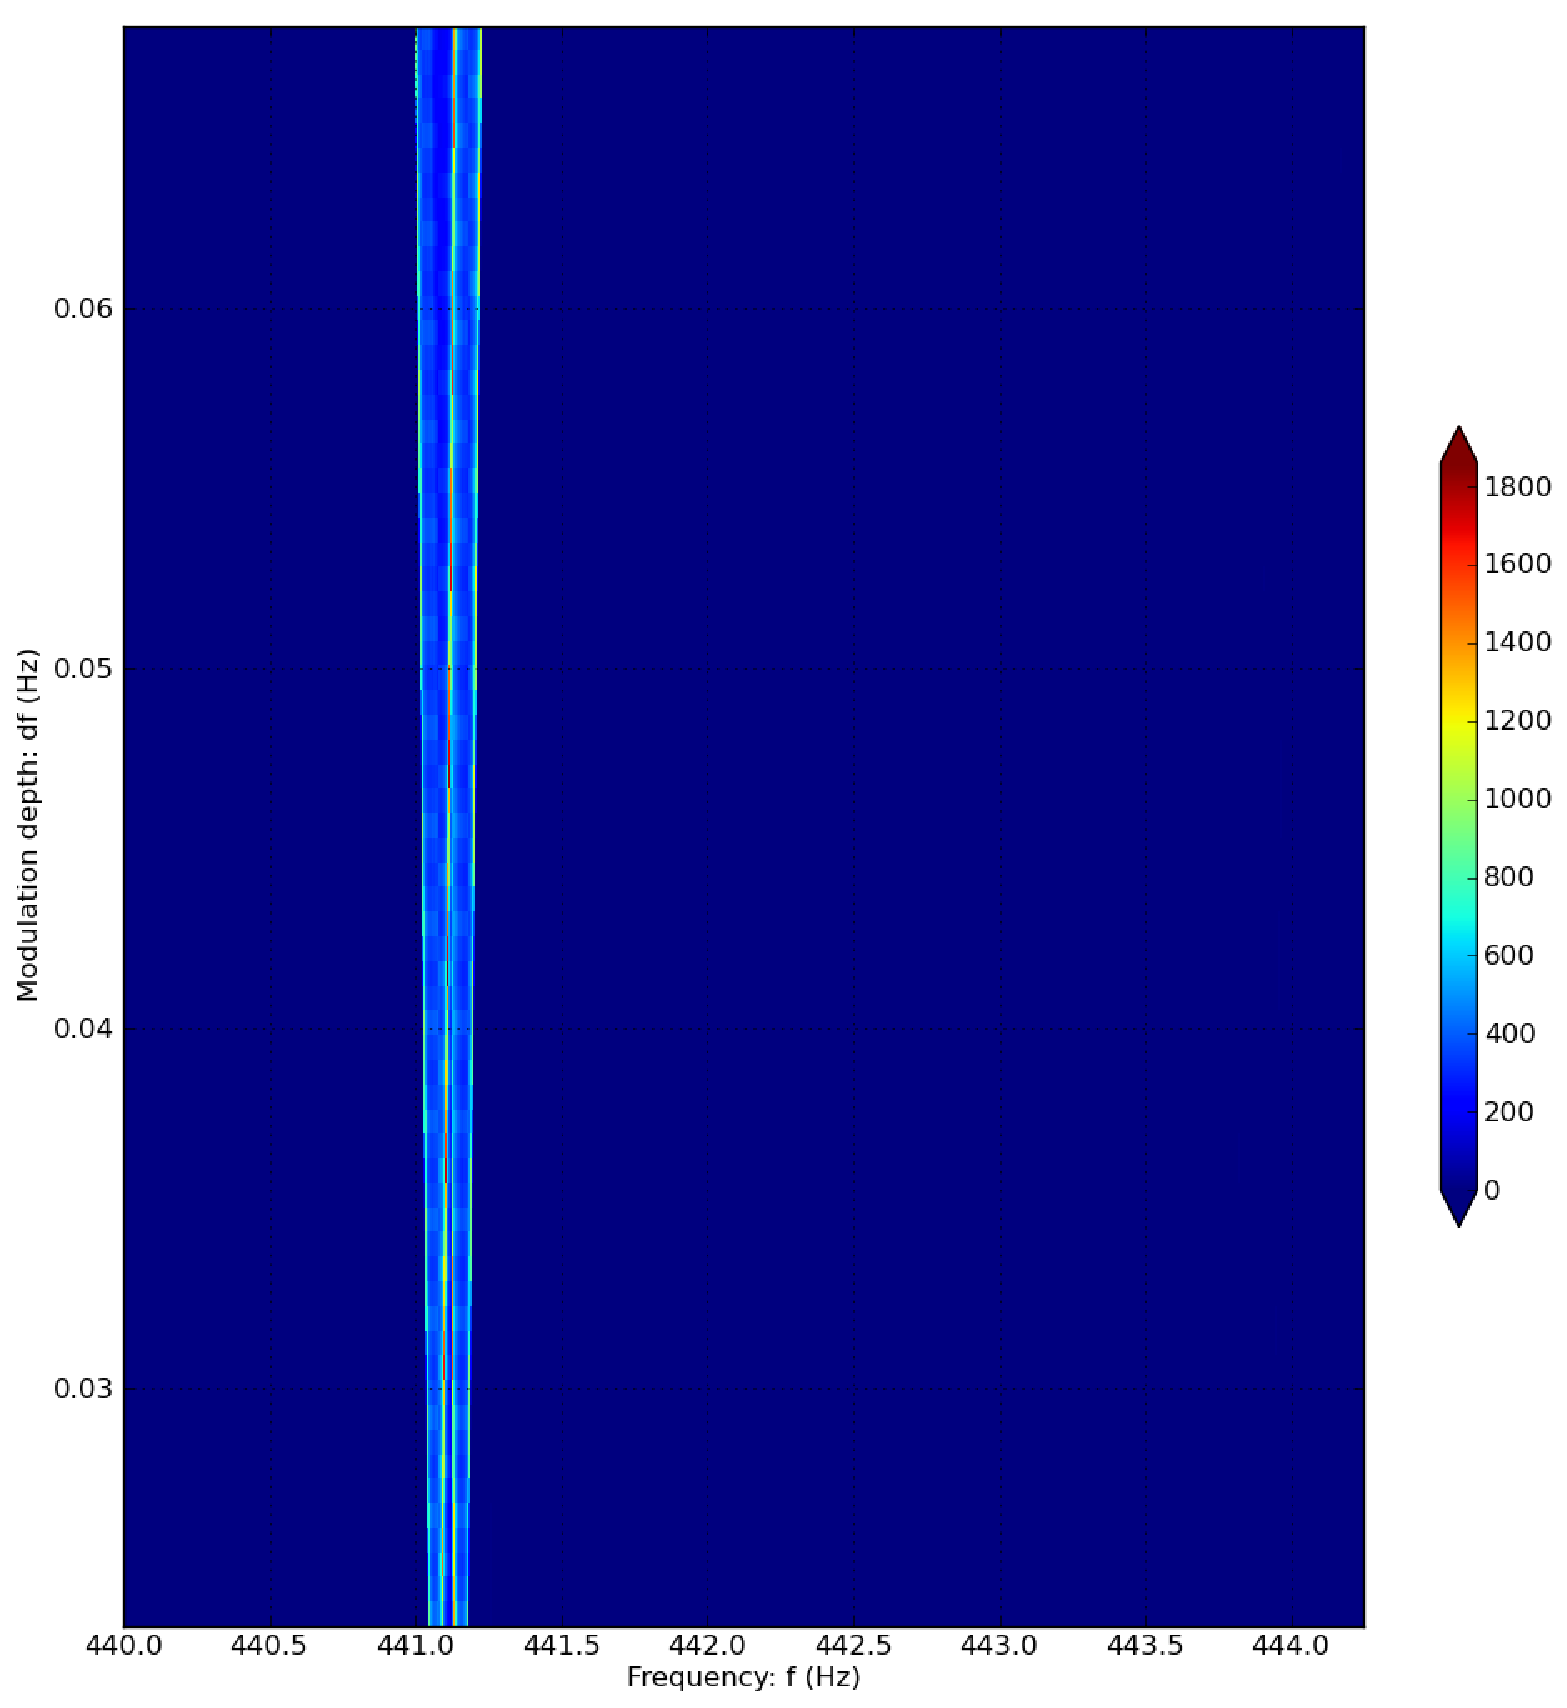
\includegraphics[width=0.8\paperwidth,height=0.62\paperheight]{bandH1-bold}}
%\end{figure}


\textbf{Scorpius X-1 MDC ``pulsar 40'' \{H1\} 5 Hz band}

p-value (based on R statistic) in red

all (frequency, modulation depth) templates


%\end{frame}

%\begin{frame}{Narrow-band heat maps in parameter space}
\subsection{Narrow-band heat maps in parameter space}


%\begin{figure}
%\protect\caption{\protect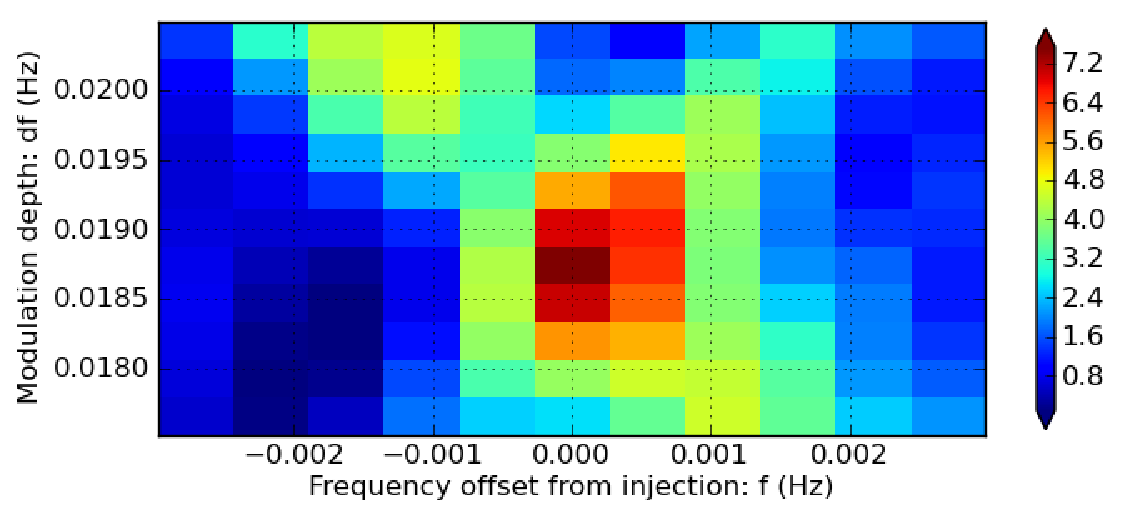
\includegraphics[width=0.4\paperwidth,height=0.2\paperheight]{heatmapH1}}
%\protect\caption{\protect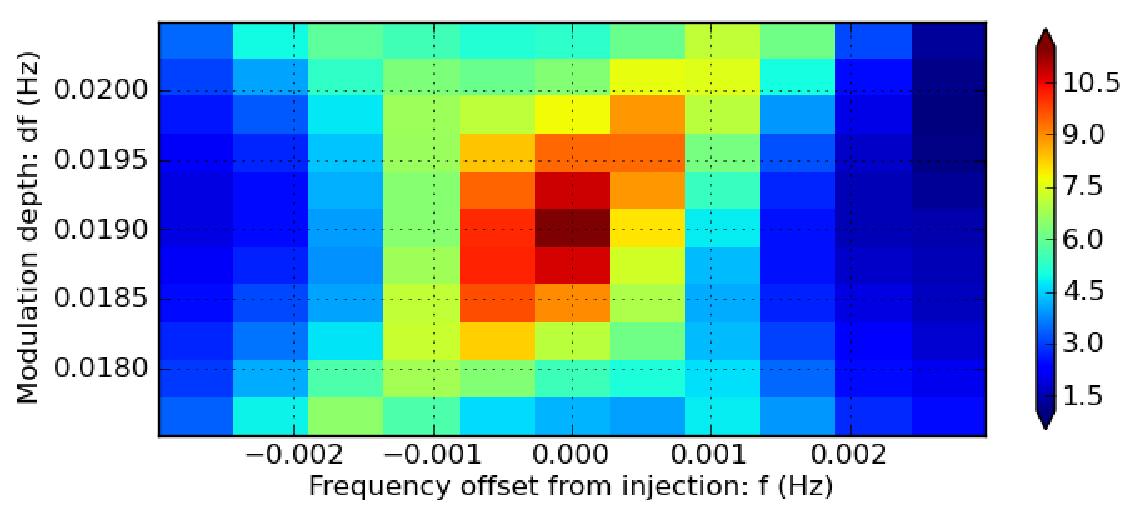
\includegraphics[width=0.4\paperwidth,height=0.2\paperheight]{heatmapL1}}
%\protect\caption{\protect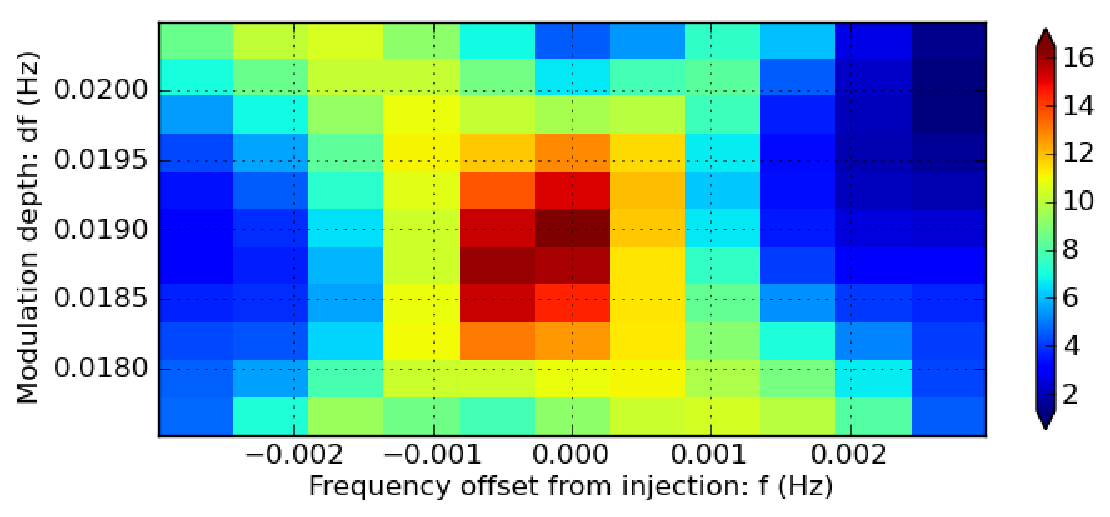
\includegraphics[width=0.4\paperwidth,height=0.2\paperheight]{heatmapV1}}
%\end{figure}


Heatmaps \{H1, L1, V1\} of 11x11 templates centered around

\textbf{Scorpius X-1 MDC ``pulsar 8''}


%\end{frame}

%\begin{frame}{Wide-band heat maps in parameter space}
\subsection{Wide-band heat maps in parameter space}


%\begin{figure}
%\protect\caption{\protect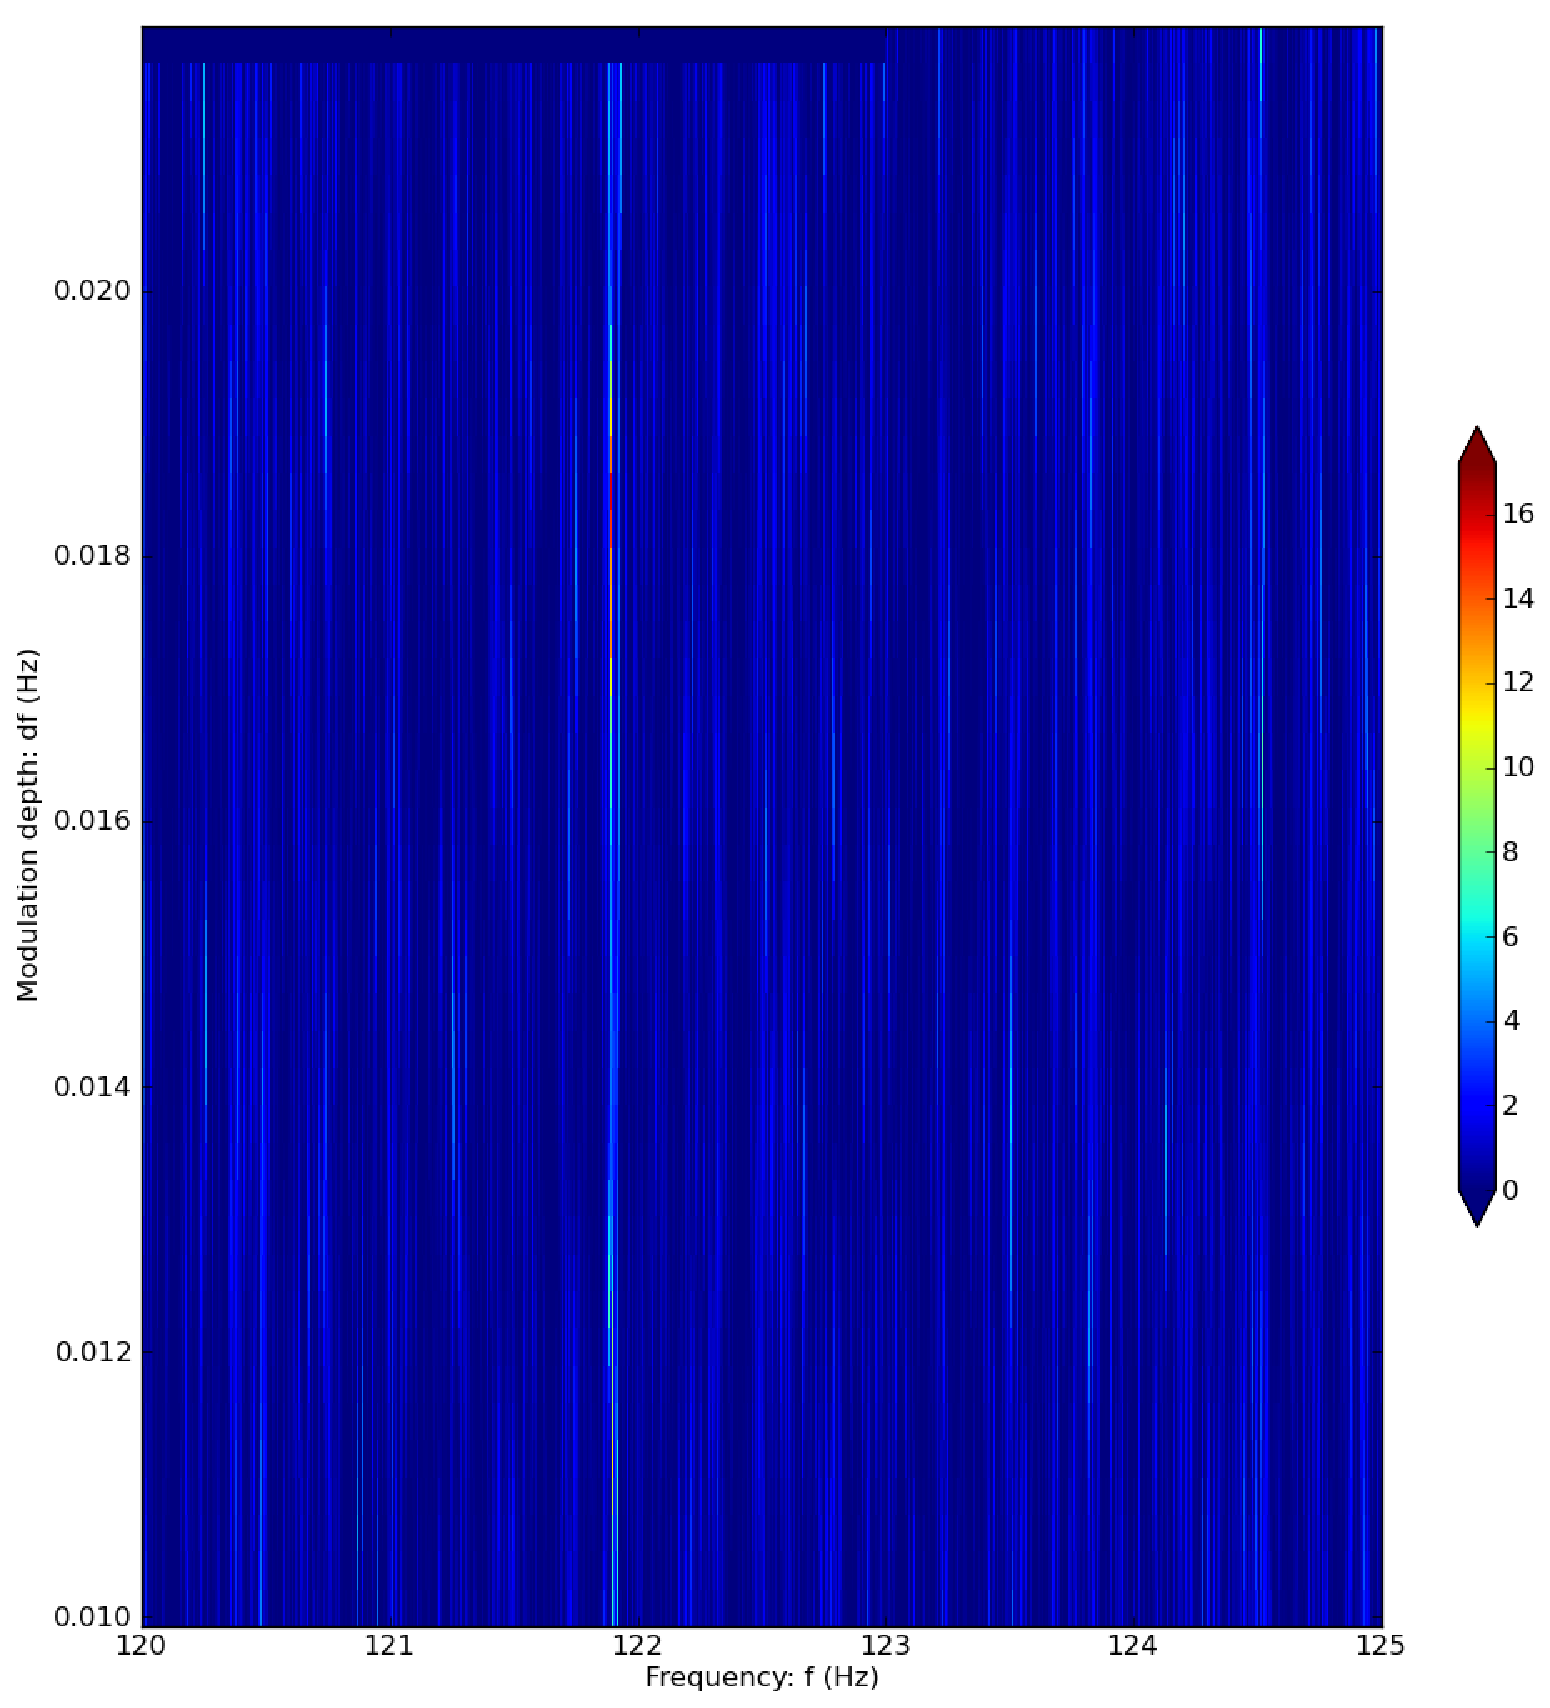
\includegraphics[width=0.8\paperwidth,height=0.62\paperheight]{bandH1}}
%\end{figure}


\textbf{Scorpius X-1 MDC ``pulsar 8'' \{H1\} 5 Hz band}

$3.6\times10^{5}$ templates, 10-22 mHz mod. depth, 120-125 Hz frequency

Signal at about (df = 0.019, f = 121.9) Hz


%\end{frame}

%\begin{frame}{Revisiting \& refining detection criteria}
\subsection{Revisiting \& refining detection criteria}


%\begin{figure}
%\protect\caption{\protect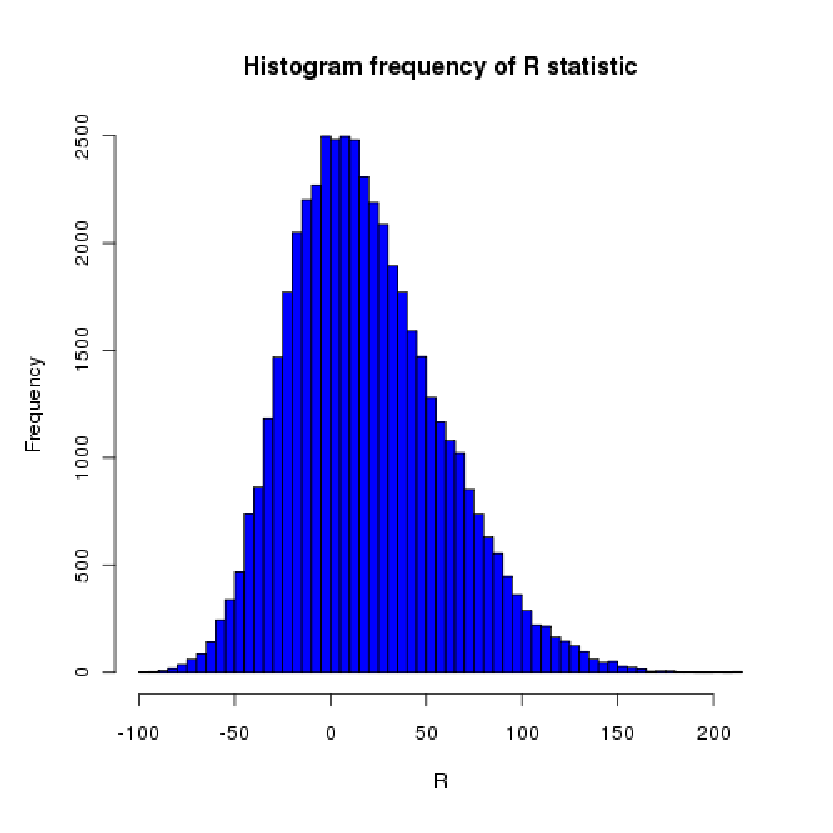
\includegraphics[width=0.45\paperwidth,height=0.45\paperheight]{StatHistRH1}\protect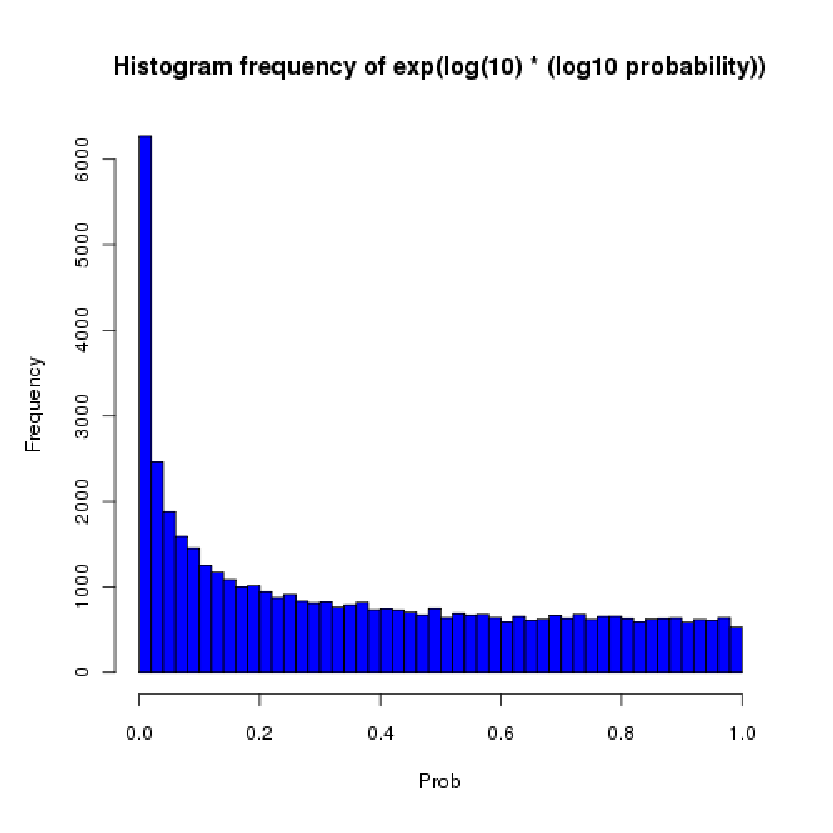
\includegraphics[width=0.45\paperwidth,height=0.45\paperheight]{StatHistProbH1}}
%\end{figure}


\textbf{Scorpius X-1 MDC statistics}

\emph{Currently refining: }plots lack full set of cuts,

\emph{understanding noise, temporal gap \& spectral leakage}

establishing signal threshold p-value $\sim$ false alarm probability
of 1\%

Re-calibrate p-values for trials factor, differences from all-sky


%\end{frame}

\section{Plans for improvement}
%\begin{frame}{Plans for improvement}

\begin{itemize}
\item \emph{Coherently combine multiple interferometer outputs: }\\
Add complex Fourier coefficients (with phase corrections)\\
to create a multi-detector statistic
\item \emph{Elliptical polarization:}\\
search antenna pattern weightings corresponding to\\
elliptical polarization -- better sensitivity
\item \emph{Orbital phase:}\\
Search over initial orbital phase by coherently combining\\
template and doubly Fourier-transformed data
\end{itemize}
%\end{frame}

\section{Summary}
%\begin{frame}{Summary}
%\subsection{General summary for TwoSpect}


\emph{Binary search summary}
\begin{itemize}
\item TwoSpect well-suited to Scorpius X-1 mock data challenges
\item Pursuing real Scorpius X-1 (and J1751-305) searches soon
\item Directed binary searches can be more sensitive with straightforward
changes
\end{itemize}

%\emph{Acknowledgments}


%Thanks to the American Physical Society for hosting this conference,
%as well as the University of Michigan, Evan Goetz for introducing
%TwoSpect, Keith Riles for guidance, and the LIGO Scientific Collaboration
%and National Science Foundation.

%\end{frame}

%\begin{frame}{Bibliography}


\emph{References}


\cite{Chakrabarty2003,GoetzThesis,GoetzTwoSpectMethods2011,PapaloizouPringle1978,Wagoner1984}


%\bibliographystyle{apsrev}
%\bibliography{bibliography}



%\part{Appendix}

%\end{frame}

%\begin{frame}{Scorpius X-1 parameters}
\subsection{Scorpius X-1 parameters}

\begin{itemize}
\item Distance: 9000 light-years (2.8 kpc)
\item Eccentricity: $<3\times10^{-3}$
\item Sky location: $\alpha$=16h19m55.1s, $\delta$=-15d38m24.9s
\item X-ray luminosity: 2.3 $\times10^{31}$W, 60000 $L_{Sol}$
\item First LIGO search: Phys. Rev. D 76 (2007) 082001; gr-qc/0605028
\item Torque-balance (Papaloizou and Pringle 1978) equation (Wagoner 1984),
generally:
\end{itemize}

\[
h_{0}=5\times10^{-27}\left(\frac{300\textup{Hz}}{\nu}\right)^{1/2}\left(\frac{F_{\times}}{10^{-8}\textup{erg cm}^{-2}\textup{s}^{-1}}\right)^{1/2}
\]

\begin{itemize}
\item Sco X-1:
\end{itemize}

\[
h_{0}=3\times10^{-26}\left(\frac{540\textup{Hz}}{f}\right)^{1/2}
\]


%\end{frame}

%\begin{frame}{Polarization addendum}
\subsection{Polarization addendum}


Also note general formula for polarization deriveable from (TwoSpect
results paper)


\[
h(t)=h_{0}F_{\times}(t,\alpha,\delta,\psi)\frac{1+\cos^{2}(\iota)}{2}\cos[\Phi(t)]+
\]



\[
h_{0}F_{+}(t,\alpha,\delta,\psi)\cos(\iota)\sin[\Phi(t)]
\]



Also: fastest known pulsar $f=$716 Hz(?)

%\end{frame}

%\begin{frame}{Sky maps using exact templates}
\subsection{Sky maps using exact templates}


%\begin{figure}
%\protect\caption{\protect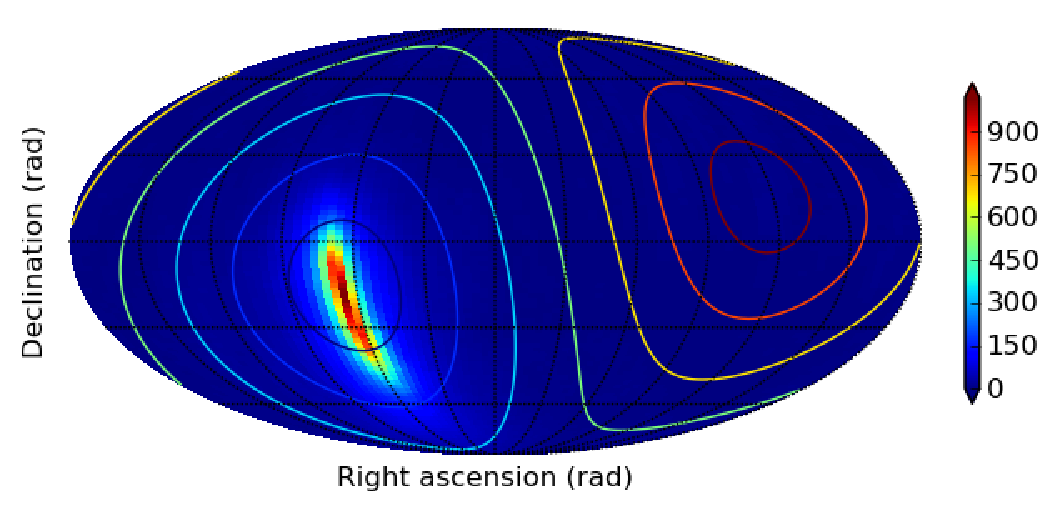
\includegraphics[width=0.4\paperwidth,height=0.2\paperheight]{maptrueH1}}
%\protect\caption{\protect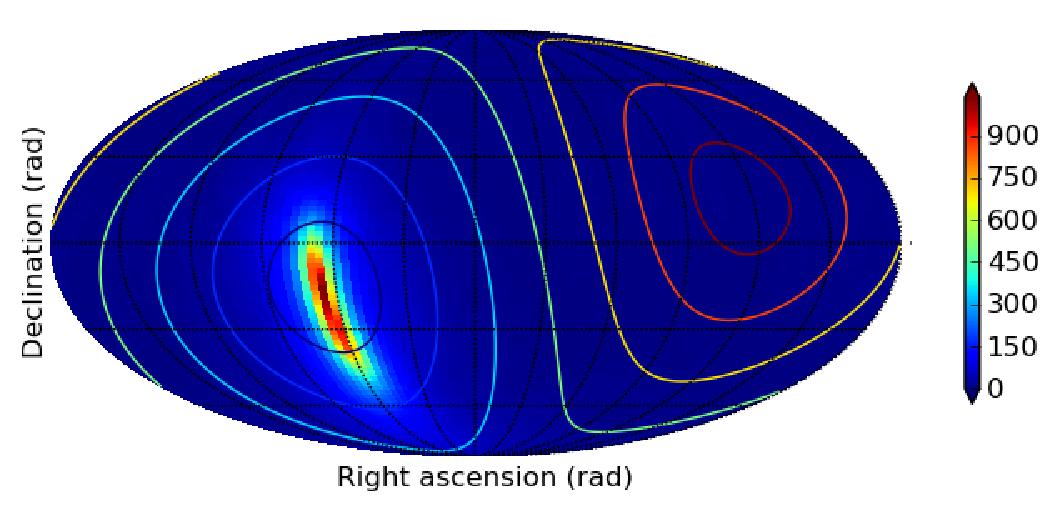
\includegraphics[width=0.4\paperwidth,height=0.2\paperheight]{maptrueL1}}
%\protect\caption{\protect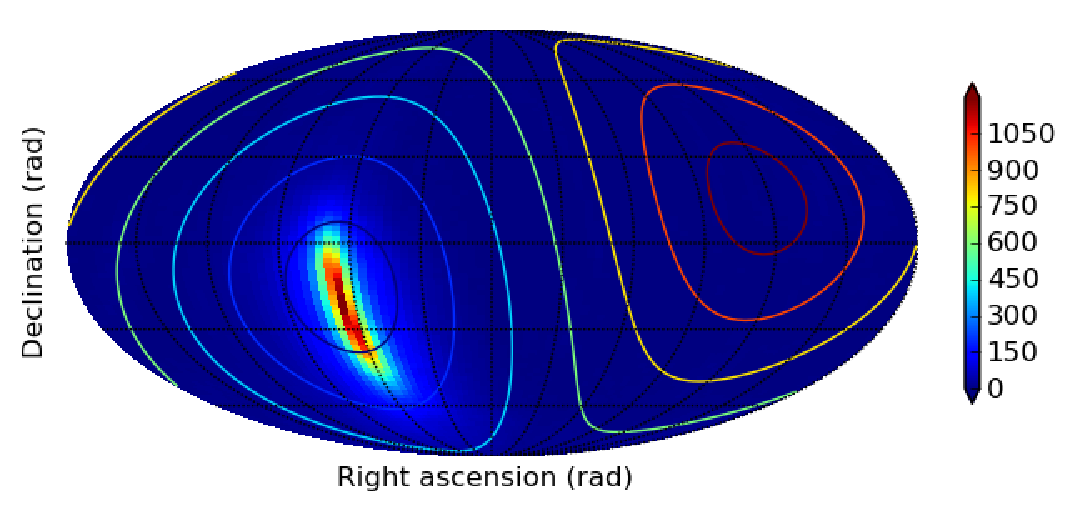
\includegraphics[width=0.4\paperwidth,height=0.2\paperheight]{maptrueV1}}
%\end{figure}


All-sky maps \{H1, L1, V1\} for fixed right ascension and declination

Scorpius X-1 mock data challenge pulsar 16 (101x101 templates)


%\end{frame}

%\begin{frame}{Coherent interferometer synthesis}
\subsection{Coherent interferometer synthesis}


\textbf{Coherent interferometer synthesis for H1-L1-V1(-?)}


\[
h(f,t)=\Sigma_{j}\left(h_{j}(f,t)+\phi_{j}(f,\alpha,\delta)\right)
\]



\[
\phi_{j}(f,\alpha,\delta)=2\pi fT_{j}(\alpha,\delta)+\phi_{0}
\]



\emph{$h_{j}(f,t)$}: complex $h$ value in SFT for interferometer
$j$, time $t$, frequency $j$


$\phi_{j}(f,\alpha,\delta)$: phase shift for right ascension $\alpha$,
declination $\delta$


(overall phase shift $\phi_{0}$ factors out: 


TwoSpect computes statistic from power)


$T_{j}(\alpha,\delta)$: time-of-flight delay between interferometers 


(projected on vector from $\alpha,\delta$)

%\end{frame}

%\begin{frame}{Circular \& elliptical polarization}
\subsection{Circular \& elliptical polarization}


\textbf{TwoSpect circular polarization assumption generalized}


Current algorithm calculates pixel powers $P$ for SFT $n$, bin $k$:


\[
\tilde{P}_{k}^{n}=\frac{F_{n}^{2}(P_{k}^{n}-<P_{k}>^{n})}{(<P_{k}>^{n})^{2}}\left[\Sigma_{n'}^{N}\frac{F_{n'}^{4}}{(<P_{k}>^{n'})^{2}}\right]^{-1}
\]



\[
F^{2}(t,\alpha,\delta)=F_{\times}^{2}(t,\alpha,\delta)+F_{+}^{2}(t,\alpha,\delta)
\]



$F$: antenna pattern polarization weighting 


as-is, assumes circular polarization


Generalize to elliptical polarization angle $\psi$ with weights $a,b$:


\[
F^{2}(t,\alpha,\delta,\psi)=aF_{\times}^{2}(t,\alpha,\delta,\psi)+bF_{+}^{2}(t,\alpha,\delta,\psi)
\]



Better upper limits; inclination angle $\iota$?

%\end{frame}

%\begin{frame}{Orbital phase \& beyond}
\subsection{Orbital phase \& beyond}


\textbf{Templates for orbital phase in the 2nd Fourier plane}
\begin{itemize}
\item Templates weight 2nd Fourier plane powers
\item Possible: phase in 2nd Fourier bins
\item Benefits: consistency between rows, binary orbital phase?
\item Significant alteration to weighting $\rightarrow$ beyond R statistic
\end{itemize}

\emph{Coherent synthesis, elliptical polarization, orbital phase}


need implementation, validation \& testing


Distributed computing (Einstein@home)?
%\end{frame}

        %---------------------------------

	%The following is an example of using the commands \textit{ref}
	%and \textit{label}. With these commands theorems, chapters,
	%sections and figurres can be labeld with names in the tex file
	%and then refered to by these names in later tex files. In
	%chapter~\ref{intro} we saw section~\ref{sample_section} or
	%theorem~\ref{sample_theorem}.

	%Lastly, here is how to include a figure. First generate an
	%encapsulated postscript file in xfig, adobe illustrator or
	%some other program. The specific commands are found in
	%\textit{chap2.tex}.

        %\begin{figure}[htb]
        %\centerline{ \epsfig{figure=sample.eps, 
        %height =  1.5 in}}
        %\caption{Sample Figure}
        %\label{sample_figure}
        %\end{figure}

